%!TEX TS-program = xetex
\documentclass{TDP005mall}
\usepackage[utf8]{inputenc}
\usepackage[swedish]{babel}
\usepackage[export]{adjustbox}
\usepackage{tabularx}
\usepackage{caption}

\usepackage[style=authoryear, backend=biber]{biblatex}
\addbibresource{reference.bib}
\usepackage{csquotes}

\renewcommand*{\contentsname}{Innehållsförteckning}

\newcommand{\version}{Version 1.1}
\author{Daniel Huber, \url{danhu849@student.liu.se}\\
  Viktor Rösler, \url{vikro653@student.liu.se}}
\title{Designspecifikation}
\date{2020-11-25}
\rhead{Daniel Huber\\
Viktor Rösler}

% For aligning captions to the left.
\captionsetup{justification=raggedright,singlelinecheck=false} 

\begin{document}
\projectpage
\tableofcontents
\newpage
\section{Revisionshistorik}
\begin{table}[!h]
\begin{tabularx}{\linewidth}{|l|X|l|}
\hline
Ver. & Revisionsbeskrivning & Datum \\\hline
1.1 & Klassdiagram och designdiskussion & 201125 \\\hline
1.0 & Designspecifikation 1:a utkast & 201125 \\\hline
\end{tabularx}
\end{table}


% TODO
% Läs CC, Primer och Design Patterns
% Notera sidor
% Skriv in Källor i dokumentet
% Skriv detaljbeskrivningarna.
% Kötta fram en diskussion.
% KLART

\section{Klassdiagram}
% Viktigaste innehållet i designspecen är ett klassdiagram som visar den objektorienterade designen av spelet.
% Klassdiagram enligt UML som beskriver hela ert system. Diagrammet skall vara kommunikativt och beskriva hela systemets inre uppbyggnad och funktion. Klassdiagrammet ska innehålla alla relationer som finns mellan era klasser. För associationer ska det framgå vilken riktning samt multiplicitet relationerna har. 

\begin{figure}[h!]
  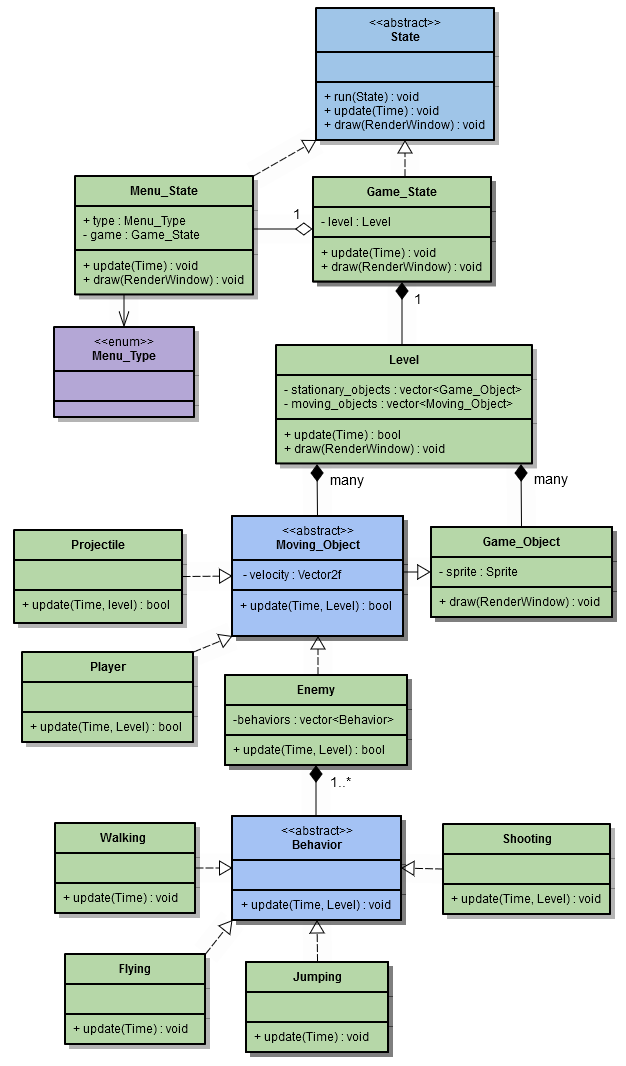
\includegraphics[height=16cm]{UML1.1.png}
  \caption{Klassdiagram\label{fig:1}}
\end{figure}

\section{Designdiskussion}% Vilka typer av spelare borde spela ert spel?
% En kort diskussion (1/2-1 sida) där ni motiverar er design och tar upp fördelar och nackdelar med den. Diskutera gärna också om det är något ni tycker är dåligt med den, och beskriv alternativa, bättre lösningar. 

% CC sida 104.

Klassen State och dess underklasser Game\_state och Menu\_State representerar tillståndet spelet befinner sig i. Endast ett state är aktivt åt gången; Game\_State om spelet är igång, eller Menu\_State om spelaren befinner sig i en meny. Ett Menu\_State innehåller ett Game\_State som ritas ut bakom menyn. Anledningen till det är att vi vill få till en snygg övergång mellan Menu\_State och Game\_State. När spelet övergår från Menu\_State till Game\_State försvinner menyn från skärmen, och nivån som ritades ut bakom menyn blir spelbar. En nackdel med att ha ett Game\_State i Menu\_State är att spelet kan behöva att läsa in fler nivåer än de som spelas. T.ex. om spelaren bläddrar i nivåmenyn ska den nivå som är markerad visas i bakgrunden, men det är inte säkert att spelaren väljer att spela den nivån. Det vore lämpligt om vi endast behöver läsa in varje nivå en gång, oavsett hur många gånger den ska användas. Det skulle kunna genomföras med en singleton-klass som har ansvaret att läsa in och komma ihåg nivåer.

Menu\_State kan representera olika sorters menyer, t.ex. en startmeny eller en pausmeny. Vilken sorts meny ett Menu\_State objekt representerar bestäms när objektet skapas. För att dölja implementationen av Menu\_State från andra klasser, och få till bra inkapsling, anropas konstruktorn till Game\_Menu med en uppräkningstyp (enumeration) som argument. Uppräkningstypen bestämmer vilken typ av meny som ska skapas.

Klassen Level representerar en nivå i spelet. Klassen innehåller två vektorer med de objekt nivån består av. Uppdelningen finns för att vi vill endast anropa en update-funktion på de objekt som behöver uppdateras under spelets gång.

% skriva om update() och draw() funktionernas kedjeanrop genom programmet här kanske?
Varje Game\_Object ritas ut genom att RenderWindow.draw() anropas med Game\_Object objektets Sprite som argument. Det fungerar för att Game\_Object ärver från sfml-klassen Drawable. Det gör att alla underklasser till Game\_Objekt också kommer kunna ritas ut. 

update() anropas i gameloopen i Game\_State som i sin tur anropar update() i Level osv. Varje objekt ska uppdatera sig självt och sedan skicka anropet vidare nedåt. varje klass ska känna till så lite som möjligt om de andra klasserna i kedjan, men Level behöver skicka sig själv vidare så att objekt av typen Moving\_Object kan veta om de kolliderar med andra objekt. spelaren/ vissa fiender behöver också känna till Level för att kunna skjuta (lägga till objekt av typen Projectile i en Level:s vektor med Moving\_Object). update() till Moving\_Object returnerar en bool för att Level ska kunna avgöra vilka objekt som ska tas bort.

Ett objekt av typen Enemy består av ett antal beteenden. Varje beteende är ett objekt av någon undertyp till den abstrakta klassen Behavior. När funktionen update anropas på ett Enemy-objekt uppdateras objektet enligt de beteenden just denna fienden har. Poängen med att bryta ut fiendernas beteenden från Enemy-klassen är att det ska vara lätt att utöka spelet med fler fiendetyper. Vi har bossfiender som ett bör-krav till projektet. Det kravet ska kunna genomföras genom att vi återanvänder, och skapar nya, beteenden till den redan existerande Enemy-klassen.  

\section{Detaljbeskrivning av klassen Player}

\section{Detaljbeskrivning av klassen Enemy}
% Detaljbeskrivning av två centrala klasser i ert spel. Den ena klassen som beskrivs ska vara den som motsvarar spelaren, den andra får ni välja själva. Detaljbeskrivningen ska innehålla följande:

%     Namn på klassen
%     Syftet med klassen
%     Vilka andra klasser som klassen har relationer till, och på vilket sätt de hänger ihop
%     En beskrivning av konstruktor(erna)
%     En beskrivning av de publika metoder som finns i klassen (get- och setmetoder kan exkluderas)
%     En beskrivning av variabler i klassen, och deras syfte

% För utkastet: Eftersom ni inte har skrivit särskilt mycket kod i projektet ännu, skriv detaljbeskrivningen utifrån frågeställningen: Hur är det tänkt att det här objektet interagerar med andra objekt i spelet? Hur kan spelaren veta när det exempelvis går in i en vägg? 

\section{Externa Filformat}
% Beskriv de externa filformat ni använt i ert spel, till exempel för highscore-listor eller banbeskrivningar. Detta är kanske inte relevant för alla, då man kan lösa uppgiften utan användning av externa format.

\newpage
\printbibliography

\end{document}

%%% Local Variables: 
%%% coding: utf-8
%%% mode: latex
%%% TeX-engine: xetex
%%% TeX-master: t
%%% End: 



